\documentclass[11pt, a4paper]{article}
\usepackage[paper=a4paper, left=1.5cm, right=1.5cm, bottom=1.5cm, top=1.5cm]{geometry}
%
\usepackage[utf8]{inputenc}
\usepackage[spanish]{babel}

% YO
\usepackage{nameref}% Only if hyperref isn't loaded
\usepackage{subfigure}

\usepackage{caratula/caratula}

%Para el uso de apéndices (nombres de la seccion)
\usepackage{appendix}
\renewcommand{\appendixtocname}{Apéndices}
\renewcommand{\appendixpagename}{Apéndices}


\begin{document}

\titulo{\center{Trabajo Práctico 2 \\ Dinámica de intercambio de opinión y el efecto de la generación de opinión en la decisión electoral.
}}
\fecha{\today}
\materia{Simulación de Eventos Discretos}

\integrante{Pedro Rodríguez}{197/12}{pedro3110.jim@gmail.com}
\integrante{Daniel J. Foguelman}{667/06}{dj.foguelman@gmail.com}
\integrante{Hernan Modrow}{767/03}{hmodrow@gmail.com}
% \integrante{Pepe Sánchez}{444/12}{pepe@gmail.com}
% \integrante{Roberto Carlos}{111/10}{roberto@gmail.com}

%Carátula
\maketitle
\newpage

%Indice
\tableofcontents
\newpage

% Demás secciones
%
\section{Introducción}
Los procesos de intercambio de opinión, donde por las interacciones interpersonales influyen en la toma de decisiones, tienen amplia aplicación en estudios de comportamiento de las personas como por ejemplo en las ciencias sociales, políticas y económicas. Dichos procesos, son de gran interés para el estudio de procesos electorales en los cuales la opinión pública tiene directa injerencia en la decisión del electorado.

En este trabajo, continuaremos el estudio del impacto de los indecisos y su interacción con otros actores de opinión más fuerte y su consecuente impacto en el resultado de una elección bi-partidista. Extenderemos este trabajo introduciendo nuevos eventos, los shocks de opinión. Estos pueden pensarse como eventos que afectan un conjunto de agentes e influyen su opinión de manera exógena. Estos cambios podrán repercutir fuertemente en su opinión.

Buscamos entonces, analizar el impacto de la influencia de los medios de información y las redes sociales en los indecisos del electorado promedio.


En el trabajo elaborado por Dima et.al encontramos dos premisas (entre otras)  sobre las cuales podemos generar un diferencial en el comportamiento de los agentes.

\begin{itemize}
    \item Las interacciones de las celdas es de a pares y unidireccional, y
    \item el vecindario está definido utilizando el vecindario von Neumann
\end{itemize}

Estas dos premisas limitan el intercambio de opiniones entre celdas alejadas entre sí. Dicho proceso, no refleja cambios de opinión cuando o bien los agentes interactúan en ámbitos nuevos o reciben información de por fuera de su núcleo de interacción.



El objeto de estudio definido por Pina et.al es de una elección entre dos
partidos (por ejemplo, en el ámbito de un ballotage presidencial), sometida a un libre
intercambio de opiniones.
Los estados posibles de un agente, se encuentran en un intervalo de valores definido en el [-3, 3]. Donde los valores de [-3, -1) pertenecen a afinidad por el partido A, los valores entre [-1, 1] denotan que el agente se encuentra en estado de indefinición mientras que los valores en el intervalo (1, 3] son del partido B.
El motivo de esto es que el grado de convicción de los sujetos se encuentra en un espectro que varía a través del tiempo.

La grilla bidimensional de los agentes será de dimensión NxN. Para definir la interacción de cada individuo, se presenta una segunda capa en la grilla la cual contiene información sobre la conectividad de cada persona (Fig. 1a). Cada sujeto modificará su estado en base a la información de la convicción de uno de sus primeros vecinos en las direcciones izquierda, derecha, arriba o abajo. Esto se define en una segunda capa de conectividad que cada determinado intervalo de tiempo genera un valor aleatorio en el rango [1, 4] que define de quien toma la influencia. A intervalos de tiempo de longitud Tau, toda la población recomputa su convicción.




\section{Modelo conceptual}
El intercambio de opinión entre personas es modelado de la siguiente manera. Las personas son modeladas mediante agentes, que en el modelo cell-devs son autómatas celulares (una celda de la grilla).
Los estados posibles de un agente representan su opinión. Dichos estados se encuentran en un intervalo de valores definido en [-3, 3]. Los valores de [-3, -1)  representan la afinidad por el partido A, los valores entre [-1, 1] denotan que el agente se encuentra en estado de indecisión mientras que los valores en el intervalo (1, 3] es afinidad hacia el partido B.
El motivo de esto es que el grado de convicción de los sujetos se encuentra en un espectro que puede variar a través del tiempo, debido a la dinámica de intercambio de opinión que se desarrolla en la población de células. Los valores más cercanos al cero representan una mayor indecisión. Mientras que los mayores en valor absoluto representan un mayor convicción o fanatismo por el partido en cuestión.

La grilla bidimensional de los agentes será de dimensión NxN. Para definir la interacción de cada individuo, se presenta una segunda capa en la grilla la cual contiene información sobre la conectividad de cada persona (ver figura \ref{fig:modelo_pina}). Cada sujeto modificará su estado en base a la información de la convicción de uno de sus primeros vecinos en las direcciones izquierda, derecha, arriba o abajo. Esto se define en una segunda capa de conectividad que cada determinado intervalo de tiempo genera un valor aleatorio en el rango [1, 4] que define de quien toma la influencia. A intervalos de tiempo de longitud Tau, toda la población recomputa su convicción.

\begin{figure}[!h]
\centering
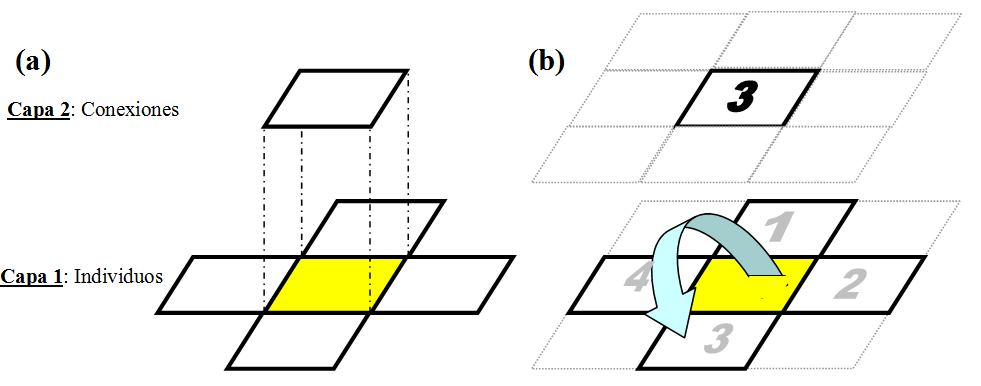
\includegraphics[scale=0.5]{imagenes/modelo_pina.png}
\caption{Vecindario de celdas utilizado para definir el comportamiento de cada agente}
\label{fig:modelo_pina}
\end{figure}

Para extender este vecindario mediante los shock de influencia, definimos modelos atómicos DEVS\cite{DEVS} externos al espacio celular que denominamos \textbf{shockers}. Estos interactúan con una cantidad fija de agentes de la grilla. En la Figura \ref{fig:modelo_shockers} observamos 3 agentes shockers interactuando con 12 celdas cada uno. Esta idea de que los atómicos interactúan con un subconjunto de la población de celdas nos permite generar esta influencia de manera dinámica. Decidimos implementar varios shockers mejorando la performance de ejecución al limitar la cantidad de puertos de salida que estos tienen. La alternativa era tener un solo modelo atómico conectado con todas las celdas de la grilla.  Con esta decisión de diseño es posible variar el tipo de influencia que genera en torno a los grupos con los que interactúa. Por ejemplo con qué periodicidad inyecta un shock, si el shock promueve la indecisión o el extremismo hacia alguno o ambos partidos.

El comportamiento de los shockers está definido de la siguiente manera.

\begin{itemize}
\item Estos atómicos no mantienen un estado.
\item Los puertos de salida están conectados con un subconjunto de las celdas y esta interconexión no varía a lo largo del tiempo. Esta primer interconexión es elegida con distribución equiprobable.
\item En cada instante de tiempo en el cual se produce un shock, para cada shocker se selecciona con probabilidad uniforme un subconjunto de puertos de salida (dentro de sus celdas dominadas) y a estas se les envía una señal.
\item La periodicidad con la cual se realiza un shock forma parte de los parámetros del modelo y está definida en relación con el Tau definido para la interacción de los agentes.
\end{itemize}

\begin{figure}[!h]
\centering
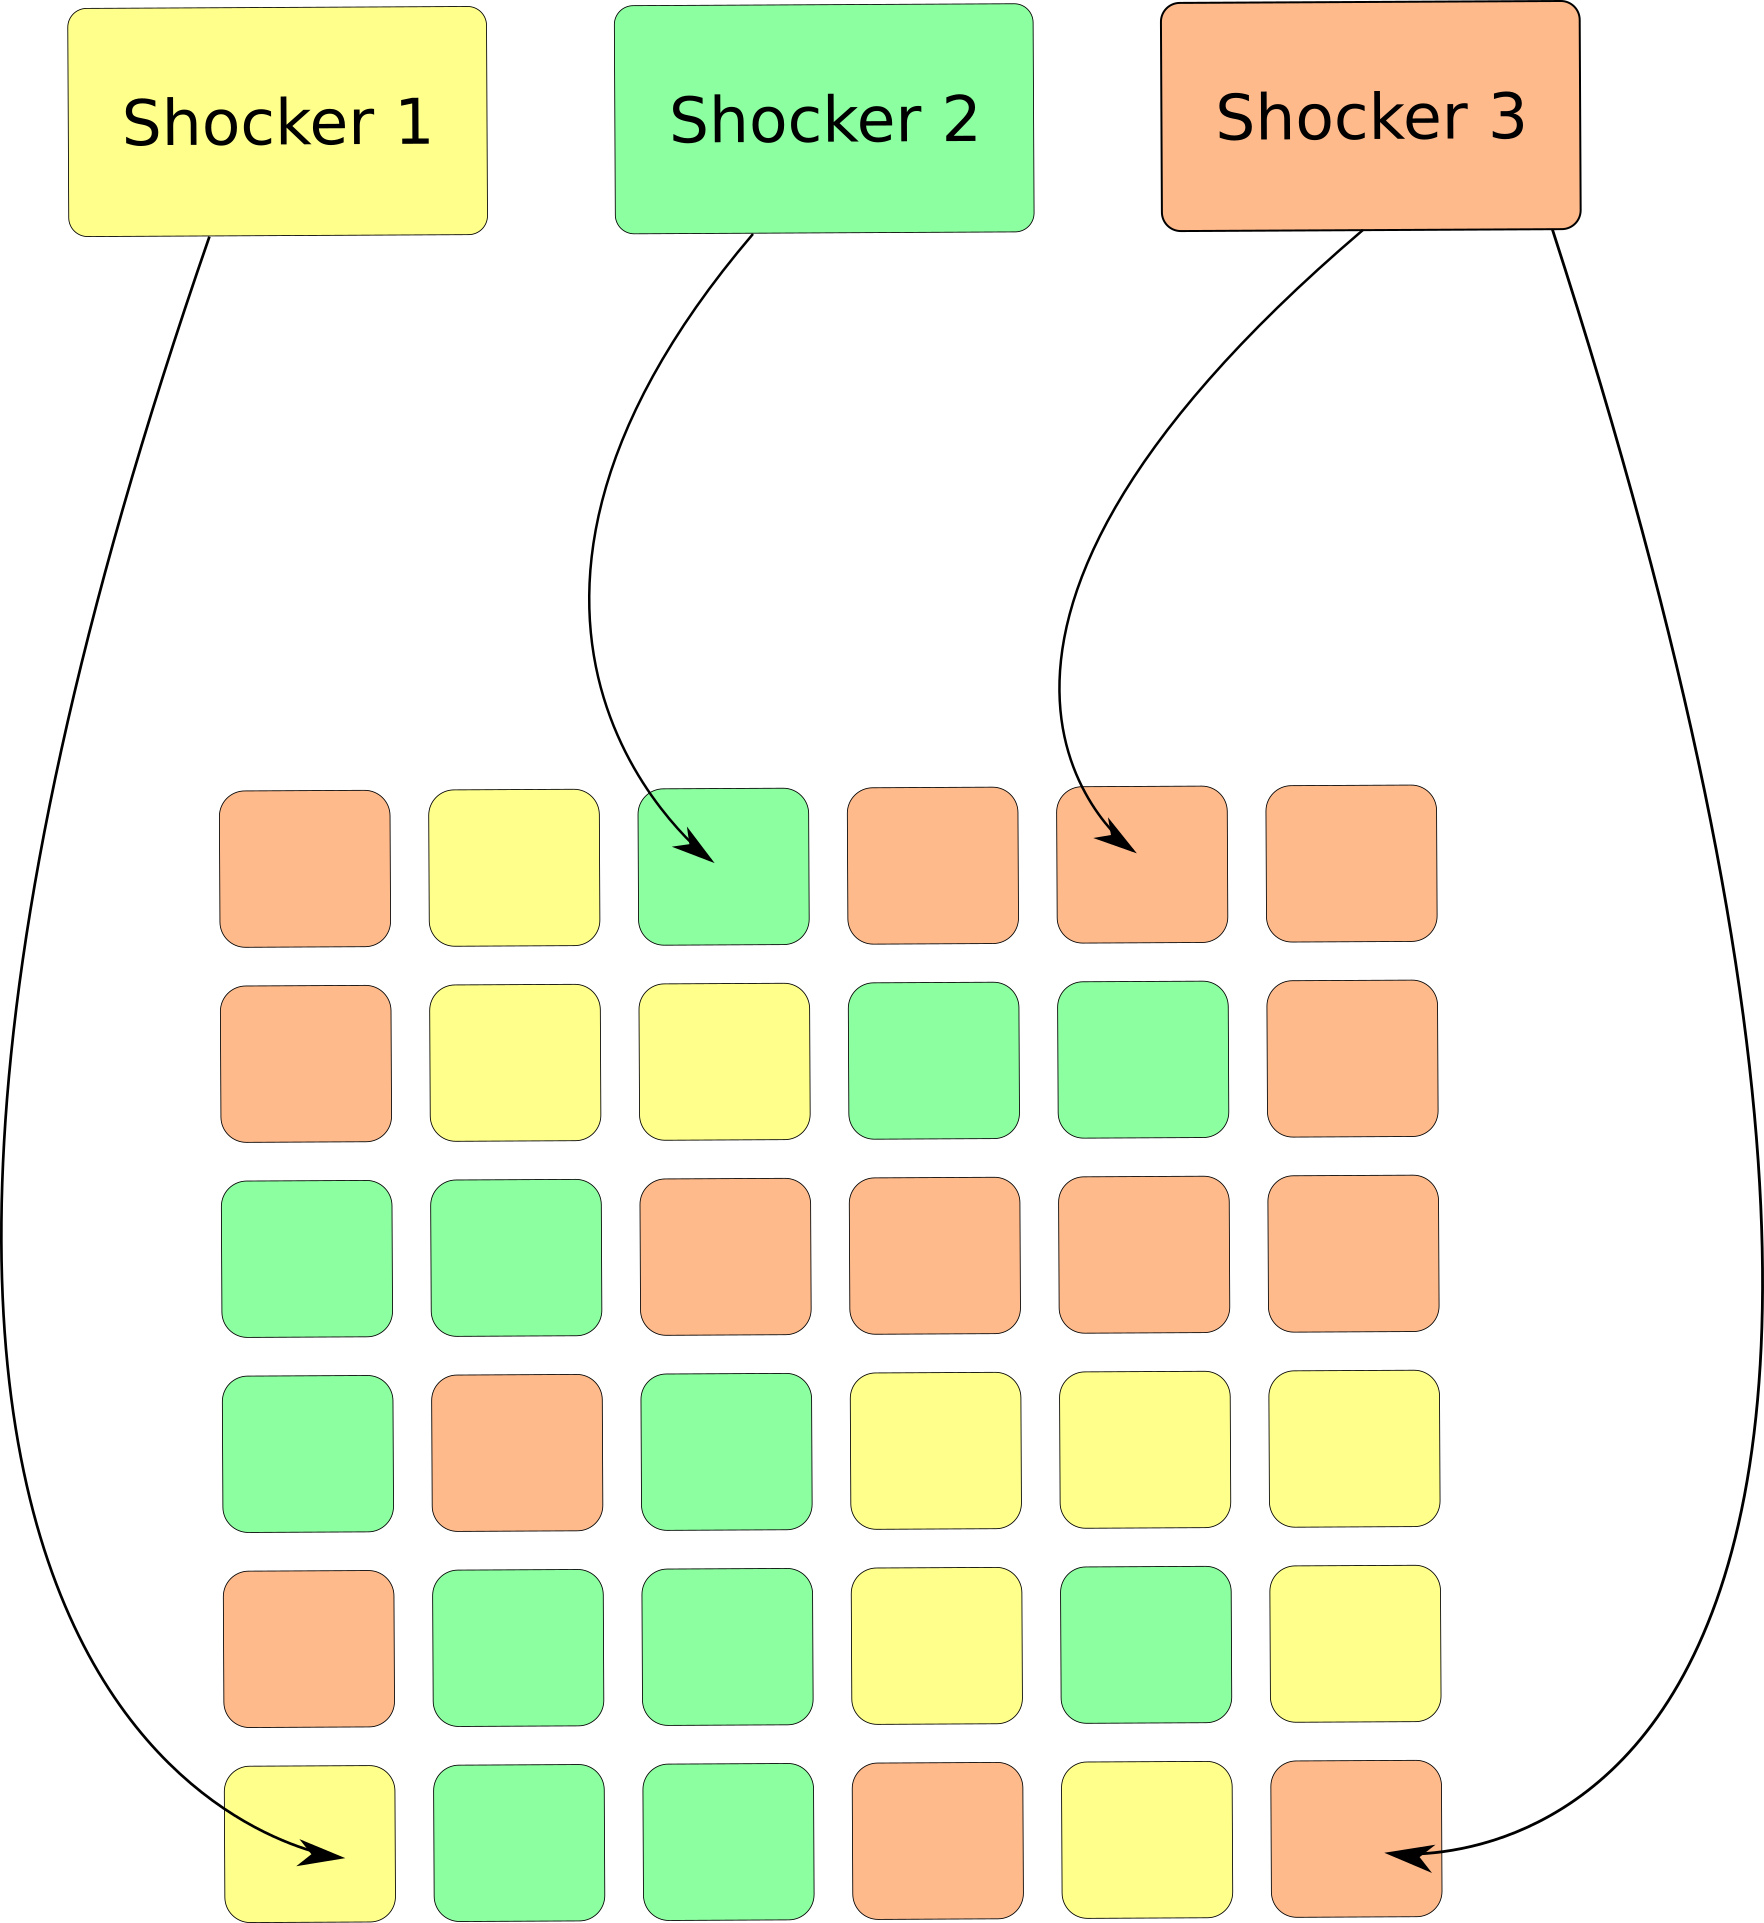
\includegraphics[scale=0.5]{imagenes/agentes_celdas_modelo.png}
\caption{Esquema que muestra el impacto de los shockers sobre el espacio celular}
\label{fig:modelo_shockers}
\end{figure}

Para los agentes, modificaremos su comportamiento. Al recibir una señal del shocker por el puerto de entrada, este definirá de manera aleatoria cómo se modifica su opinión y con distribución uniforme se polarizará o se indecidirá según el tipo de shock que lo afecte.

\begin{itemize}
    \item[] rule : { if ( (0,0,0) < 0 , uniform(-3, -2), uniform(2, 3) ) } 0 { (0,0,0) = 5 }
    \item[] rule : { if ( (0,0,0) < 0 , uniform(-1, 0), uniform(0, 1) ) } 0 { (0,0,0) = 6 }
\end{itemize}





\section{Desarrollo}
Para desarrollar el traductor de \texttt{XMILE} a \texttt{DEVSML}, del cual se habló en la sección anterior, decidimos basarnos en 2 (dos) modelos clásicos implementados en \textit{System Dynamics}. 

Estos modelos son: 
\begin{description}
	\item[Teacup] que modela una taza de café en una habitación, que se enfría progresivamente hasta alcanzar la temperatura ambiente
	\item[SIR] 	que modela una población que sucumbe ante una infección que se propaga en la misma, y posteriormente se va recuperando, hasta que no queda ningún infectado
\end{description}

Mediante el estudio de estos dos modelos, analizamos como los diferentes elementos de cada archivo \texttt{XMILE} pueden ser traducidos a un modelo acoplado en DEVS  de forma tal que esta traducción pueda ser ejecutada. 
Partiendo de un modelo escrito en \texttt{XMILE}, transformandolo en un modelo DEVS con formato \texttt{DEVSML} para luego ejecutarlo utilizando el simulador \textit{CD++}. Finalmente replicando los resultados que se obtienen con simuladores de \textit{System Dynamics}.


A continuación, exponemos cada uno de los modelos mencionados, mencionando cómo nos ayudaron en el desarrollo del traductor. 

Aprovecharemos que el modelo \textit{Teacup} traducido contiene pocos archivos para mostrar el código generado por el traductor. Para la exposición del comportamiento de los otros modelos cuya traducción genera una mayor cantidad de archivos, utilizaremos el lenguage formal típico con que se expresan modelos DEVS.

% (http://pysd.readthedocs.io/en/master/)
En el proceso de investigación realizado en este trabajo, encontramos la herramienta \textit{PySD}\cite{pysd}, que permite simular modelos \textit{Vensim} el lenguaje Python, simplificando de forma considerable el análisis y las corridas de los modelos \texttt{SD} y su comparación con los modelos \textit{CD++} correspondientes efectuados en el TP.


\section{Resultados}
%TODO Armar seccion con los graficos 

\section{Conclusiones y Trabajo futuro}
%TODO Completar con todas las cosas que quedaron afuera.

\section{Referencias}
\begin{thebibliography}{9}

\bibitem{xmile}
  Adler, Steve. \textit{XMILE: System Dynamics Standard @ OASIS}. July 2013.   \url{https://www.ibm.com/developerworks/community/blogs/adler/entry/xmile_system_dynamics_standard_oasis?lang=en}

\bibitem{devs76}
  Zeigler, B. P. \textit{Theory of Modeling and Simulation}. John Wiley, 1976.

\bibitem{devsml}
  Mittal, S., J.L. Risco-Martín and B.P. Zeigler. \textit{DEVSML: automating DEVS execution over SOA towards transparent simulators.}. In M.J. Ades (ed.), Spring Simulation Multiconference, SpringSim 2007, Norfolk, VA, pp. 287-295

\bibitem{qss}
 F. Cellier, E. Kofman. \textit{Continuous System Simulation}. Springer, New York, 2006.

\bibitem{xml}
  XML. \url{http://www.w3.org/XML/}
 
\bibitem{pysd}
 PySD: Simulating System Dynamics Models in Python. \urk{http://pysd.readthedocs.io/en/master/}
 
\bibitem{muparser}
 muparser: Fast Math Parser Library. \url{http://beltoforion.de/article.php?a=muparser}




\end{thebibliography}


%
% \section{Conclusiones}
% Durante el desarrollo de este Trabajo Práctico, tuvimos que aprender a utilizar varias herramientas necesarias para la realización del mismo. Entre las más importantes podemos destacar las siguientes:
\begin{itemize}
\item entender el formalismo DEVS y aplicarlo a problemas concretos mediante la utilización del Simulador Avanzado \textit{CD++} desarrollado parcialmente por ex-alumnos de la materia
\item entender el formalismo \textit{System Dynamics} (\texttt{SD}), su capacidad para modelar sistemas de ecuaciones diferenciales continuos, y su relación y punto de contacto con el formalismo DEVS, para poder así reescribir uno modelo de un formalismo al otro
\item tuvimos la necesidad de entender el funcionamiento de los módulos \texttt{QSS}(\textit{Quantized State System}), que utilizamos como integradores en nuestro sistema
\item aplicamos técnicas de \textit{parsing} y transformación de documentos así como también \textit{templates} para simplificar el proceso de traducción de modelos en formato \texttt{XMILE} y formato \texttt{DEVSML} y también para interpretar los \textit{logs} generados por el simulador \textit{CD++}
\item técnicas de visualización para poder comparar eficientemente el \textit{output} generado por el modelo original y por su traducción para los mismos \textit{inputs}
\end{itemize}

A partir de la aplicación de todo lo expuesto más arriba, pudimos ver cómo es posible traducir de forma automática modelos simples (en nuestro caso el modelo \textit{Teacup} y el modelo \textit{SIR}) \textit{System Dynamics} en model DEVS, de forma tal que los resultados de su ejecución para los mismos \textit{inputs} sean cualitativamente iguales, y cuantitativamente casi idénticos.

Con los resultados finales obtenidos, podemos decir que hemos desarrollado exitosamente un traductor simple y básico, que permite traducir de forma automática modelos básico de \textit{System Dynamics} en DEVS, que es un formalismo que al ser basado en eventos discretos, permite incluir en estos modelos variaciones no continuas (que podríamos llamar \textit{eventos}) en el valor de las variables de un modelo en el medio de una simulación de forma natural. De esta forma, la representación de dichos modelos en el formalismo DEVS, permite enriquecer la expresividad del modelo original.
%
\clearpage
\addappheadtotoc
\appendix
\appendixpage

\subsection{Teacup}
A modo de completitud mostramos la definición formal de los modelos atómicos 
utilizados en el acoplado \texttt{Top}, con la descripción de su comportamiento interno.
\begin{itemize}
	
	\item \textbf{Cte} : $ roomTemperature, characteristicTime \rightarrow \langle X, S, Y, \delta_{int}, \delta_{ext}, \lambda, t_{a} \rangle$ \newline
	\begin{itemize}
		\item $ X = \{ inValue \} $ \newline
		\item $ S = \{ value \} $ \newline
		\item $ Y = \{ out \} $ \newline
		\item $ \delta_{int}(\langle value \rangle) = \emptyset $ \newline
		\item $ \delta_{ext} (\langle value \rangle, e, x)= \{ value := x.value \} $ \newline
		\item $ \lambda(\langle value \rangle, out) = value $ \newline
		\item $ t_{a}(s) = \infty $ 
	\end{itemize}
	
	\item \textbf{Fminus} : $ fmTeacupTemperatureHeatLossToRoom \rightarrow \langle X, S, Y, \delta_{int}, \delta_{ext}, \lambda, t_{a} \rangle$ \newline
	\begin{itemize}
		\item $ X = \{ inRoomTemperature, inCharacteristicTime, inTeacupTemperatureIntegrator \} $ \newline
		\item $ S = \{ roomTemperature, characteristicTime, teacupTemperatureIntegrator, isSetRoomTemperature, \newline isSetCharacteristicTime, isSetTeacupTemperatureIntegrator \} $ \newline
		\item $ Y = \{ out \} $ \newline
		\item $ \delta_{int}(s) = \emptyset $ \newline
		\item $ \delta_{ext}(s, e, x) = \{
		\\if (x.port = inRoomTemperatureroomTemperature) roomTemperature := x.value; isSetRoomTemperature := true
		\\if (x.port = inCharacteristicTime) characteristicTime := x.value; isSetCharacteristicTime := true
		\\if (x.port = inTeacupTemperatureIntegrator) teacupTemperatureIntegrator = x.value; \\isSetTeacupTemperatureIntegrator := true 
		\} $ \newline
		\item $ \lambda(s, out) = if(todas \ las \ variables \ seteadas) \{ 
		\\(teacupTemperatureIntegrator-roomTemperature)/characteristicTime\} \ else \ \emptyset$ \newline
		\item $ t_{a} = \infty $ 
	\end{itemize}
	
	\item \textbf{Ftot} : $ ftTeacupTemperature \rightarrow \langle X, S, Y, \delta_{int}, \delta_{ext}, \lambda, t_{a} \rangle$ \newline
	\begin{itemize}
		\item $ X = \{ inMinusHeatLossToRoom \} $ \newline
		\item $ S = \{ plus, minus \} $ \newline
		\item $ Y = \{ out \} $ \newline
		\item $ \delta_{int}(\langle plus, minus \rangle) = \emptyset $ \newline
		\item $ \delta_{ext}(\langle plus, minus \rangle, e, x) = \{ 
		\\if (x.port = inPlus) plus := x.value
		\\if (x.port == inMinusHeatLossToRoom) minus := x.value
		\} $ \newline
		\item $ \lambda(\langle plus, minus \rangle, out) = (plus - minus) $ \newline
		\item $ t_{a} = \infty $ 
	\end{itemize}
	\item \textbf{QSS1} : $ teacupTemperatureIntegrator \rightarrow \langle X, S, Y, \delta_{int}, \delta_{ext}, \lambda, t_{a} \rangle$ \newline
	\begin{itemize}
		\item $ X = \{ in \} $ \newline
		\item $ S = \{ ? \} $ \newline
		\item $ Y = \{ out \} $ \newline
		\item $ \delta_{int}(s) = \{ ? \} $ \newline
		\item $ \delta_{ext}(s, e, x) = \{ ? \} $ \newline
		\item $ \lambda(s) = ? $ \newline
		\item $ t_{a} = \{ ? \} $ 
	\end{itemize}
\end{itemize}

Ahora que ya tenemos lo atómicos, expresamos el acoplado que utiliza a los atómicos expuestos más arriba:
\begin{itemize}
	\item $ Top \rightarrow \langle X, Y, \{ M_{1}, M_{2}, M_{3}, M_{4}, M_{5} \}, C_{xx}, C_{yx}, C_{yy}, Select \rangle$ \newline
	\begin{itemize}
		\item $ X = \{ \} $ \newline
		\item $ Y = \{ \} $ \newline
		\item $ M_{1} = roomTemperature $ \newline
		\item $ M_{2} = characteristicTime $ \newline
		\item $ M_{3} = fmTeacupTemperatureHeatLossToRoom$ \newline
		\item $ M_{4} = ftTeacuptTemperature $ \newline
		\item $ M_{5} = teacupTemperatureIntegrator $ \newline
		\item $ C_{xx} = $ \{ \} \newline
		\item $ C_{yx} = \{ (M_{1}.!out, M_{3}.?inRoomTemperture), (M_{2}.!out, M_{3}.?inCharacteristicTime), \\
		(M_{5}.!out, M_{3}.?inTecupTemperatureIntegrator), (M_{3}.!out, M_{4}.?inMinusHeatLossToRoom), \\
		(M_{4}.!out, M_{5}.?in) \} $ \newline
		\item $ C_{yy} = \{ \} $ \newline
	\end{itemize}
\end{itemize}


\subsection{SIR}
A continuación, exponemos formalmente los modelos atómicos utilizados en el acoplado Top, con la descripción de su comportamiento interno.
\begin{itemize}
\item \textbf{Cte} : $ totalPopulation, contactInfectivity, duration \rightarrow \langle X, S, Y, \delta_{int}, \delta_{ext}, \lambda, t_{a} \rangle$ \newline
$ X = \{ inValue \} $ \newline
$ S = \{ value \} $ \newline
$ Y = \{ out \} $ \newline
$ \delta_{int}(\langle value \rangle) = \emptyset $ \newline
$ \delta_{ext} (\langle value \rangle, e, x)= \{ value := x.value \} $ \newline
$ \lambda(\langle value \rangle, out) = value $ \newline
$ t_{a}(s) = \infty $

\item \textbf{Fminus} : $ fmSusceptiblesSuccumbing \rightarrow \langle X, S, Y, \delta_{int}, \delta_{ext}, \lambda, t_{a} \rangle$ \newline
$ X = \{ inTotalPopulation, inContactInfectivity, inInfectedIntegrator, inSuceptiblesIntegrator \} $ \newline
$ S = \{ totalPopulation, contactInfectivity, infectedIntegrator, suceptiblesIntegrator, isSetTotalPopulation, \newline isSetContactInfectivity, isSetInfectedIntegrator, isSetSuceptiblesIntegrator \} $ \newline
$ Y = \{ out \} $ \newline
$ \delta_{int}(s) = \emptyset $ \newline
$ \delta_{ext}(s, e, x) = \{
\\if (x.port = inTotalPopulation) totalPopulation := x.value; isSetTotalPopulation := true
\\if (x.port = inContactInfectivity) contactInfectivity := x.value; isSetContactInfectivity := true
\\if (x.port = inInfectedIntegrator) infectedIntegrator = x.value; \\isSetInfectedIntegrator := true 
\\if (x.port = inSuceptiblesIntegrator) suceptiblesIntegrator = x.value; \\isSetSuceptiblesIntegrator := true
\} $ \newline
$ \lambda(s, out) = if(todas \ las \ variables \ seteadas) \{ 
\\susceptiblesIntegrator*infectedIntegrator/totalPopulation*contactInfectivity\} \ else \ \emptyset$ \newline
$ t_{a} = \infty $ 

\item \textbf{Fplus} : $ fpInfectedSuccumbing \rightarrow \langle X, S, Y, \delta_{int}, \delta_{ext}, \lambda, t_{a} \rangle$ \newline
$ X = \{ inTotalPopulation, inContactInfectivity, inInfectedIntegrator, inSuceptiblesIntegrator \} $ \newline
$ S = \{ totalPopulation, contactInfectivity, infectedIntegrator, suceptiblesIntegrator, isSetTotalPopulation, \newline isSetContactInfectivity, isSetInfectedIntegrator, isSetSuceptiblesIntegrator \} $ \newline
$ Y = \{ out \} $ \newline
$ \delta_{int}(s) = \emptyset $ \newline
$ \delta_{ext}(s, e, x) = \{
\\if (x.port = inTotalPopulation) totalPopulation := x.value; isSetTotalPopulation := true
\\if (x.port = inContactInfectivity) contactInfectivity := x.value; isSetContactInfectivity := true
\\if (x.port = inInfectedIntegrator) infectedIntegrator = x.value; \\isSetInfectedIntegrator := true 
\\if (x.port = inSuceptiblesIntegrator) suceptiblesIntegrator = x.value; \\isSetSuceptiblesIntegrator := true
\} $ \newline
$ \lambda(s, out) = if(todas \ las \ variables \ seteadas) \{ 
\\susceptiblesIntegrator*infectedIntegrator/totalPopulation*contactInfectivity\} \ else \ \emptyset$ \newline
$ t_{a} = \infty $ 

\item \textbf{Fminus} : $ fmInfectedRecovering \rightarrow \langle X, S, Y, \delta_{int}, \delta_{ext}, \lambda, t_{a} \rangle$ \newline
$ X = \{ inDuration, inInfectedIntegrator \} $ \newline
$ S = \{ duration, infectedIntegrator, isSetDuration, isSetInfectedIntegrator \} $ \newline
$ Y = \{ out \} $ \newline
$ \delta_{int}(s) = \emptyset $ \newline
$ \delta_{ext}(s, e, x) = \{
\\if (x.port = inDuration) duration := x.value; isSetDuration := true
\\if (x.port = inInfectedIntegrator) infectedIntegrator = x.value; \\isSetInfectedIntegrator := true 
\} $ \newline
$ \lambda(s, out) = if(todas \ las \ variables \ seteadas) \{ 
\\infectedIntegrator/duration\} \ else \ \emptyset$ \newline
$ t_{a} = \infty $ 

\item \textbf{Fplus} : $ fpRecoveredRecovering \rightarrow \langle X, S, Y, \delta_{int}, \delta_{ext}, \lambda, t_{a} \rangle$ \newline
$ X = \{ inDuration, inInfectedIntegrator \} $ \newline
$ S = \{ duration, infectedIntegrator, isSetDuration, isSetInfectedIntegrator \} $ \newline
$ Y = \{ out \} $ \newline
$ \delta_{int}(s) = \emptyset $ \newline
$ \delta_{ext}(s, e, x) = \{
\\if (x.port = inDuration) duration := x.value; isSetDuration := true
\\if (x.port = inInfectedIntegrator) infectedIntegrator = x.value; \\isSetInfectedIntegrator := true 
\} $ \newline
$ \lambda(s, out) = if(todas \ las \ variables \ seteadas) \{ 
\\infectedIntegrator/duration\} \ else \ \emptyset$ \newline
$ t_{a} = \infty $

\item \textbf{Ftot} : $ ftSuceptibles, ftInfected, ftRecovered \rightarrow \langle X, S, Y, \delta_{int}, \delta_{ext}, \lambda, t_{a} \rangle$ \newline
$ X = \{ inMinus, inPlus \} $ \newline
$ S = \{ plus, minus \} $ \newline
$ Y = \{ out \} $ \newline
$ \delta_{int}(\langle plus, minus \rangle) = \emptyset $ \newline
$ \delta_{ext}(\langle plus, minus \rangle, e, x) = \{ 
\\if (x.port = inPlus) plus := x.value
\\if (x.port == inMinus) minus := x.value
\} $ \newline
$ \lambda(\langle plus, minus \rangle, out) = (plus - minus) $ \newline
$ t_{a} = \infty $ 


\item \textbf{QSS1} : $ susceptiblesIntegrator, infectedIntegrator, recoveredIntegrator  \rightarrow \langle X, S, Y, \delta_{int}, \delta_{ext}, \lambda, t_{a} \rangle$ \newline
$ X = \{ in \} $ \newline
$ S = \{ ? \} $ \newline
$ Y = \{ out \} $ \newline
$ \delta_{int}(s) = \{ ? \} $ \newline
$ \delta_{ext}(s, e, x) = \{ ? \} $ \newline
$ \lambda(s) = ? $ \newline
$ t_{a} = \{ ? \} $ 
\end{itemize}

El acoplado que utiliza los atómicos expuestos más arriba es:

% TODO modificar el acoplado para darle forma al acoplado de SIR
\begin{itemize}
	\item $ Top \rightarrow \langle X, Y, \{ M_{1}, M_{2}, M_{3}, M_{4}, M_{5} \}, C_{xx}, C_{yx}, C_{yy}, Select \rangle$ \newline
	$ X = \{ \} $ \newline
	$ Y = \{ \} $ \newline
	$ M_{1} = totalPopulation $ \newline
	$ M_{2} = contactInfectivity $ \newline
	$ M_{3} = duration $ \newline
	$ M_{4} = fmSusceptiblesSuccumbing $ \newline
	$ M_{5} = ftSuceptibles  $ \newline
	$ M_{6} = susceptiblesIntegrator  $ \newline
	$ M_{7} = fpInfectedSuccumbing $ \newline
	$ M_{8} = fmInfectedRecovering  $ \newline
	$ M_{9} = ftInfected  $ \newline
	$ M_{10} = infectedIntegrator  $ \newline
	$ M_{11} = fpRecoveredRecovering  $ \newline
	$ M_{12} = ftRecovered  $ \newline
	$ M_{13} = recoveredIntegrator  $ \newline
	$ C_{xx} = $ \{ \} \newline
	$ C_{yx} = \{ (M_{1}.!out, M_{4}.?inTotalPopulation), (M_{1}.!out, M_{5}.?inTotalPopulation), \\
	(M_{2}.!out, M_{4}.?inContactInfectivity), (M_{2}.!out, M_{5}.?inContactInfectivity), \\
	(M_{3}.!out, M_{6}.?inDuration), (M_{3}.!out, M_{7}.?inDuration), \\
	(M_{4}.!out, M_{5}.?inMinus), (M_{5}.!out, M_{6}.?in), \\
	(M_{6}.!out, M_{4}.?inSusceptiblesIntegrator), (M_{6}.!out, M_{7}.?inSuceptiblesIntegrator), \\
	(M_{7}.!out, M_{9}.?inPlus), (M_{8}.!out, M_{9}.?inMinus), \\
	(M_{9}.!out, M_{10}.?in), (M_{10}.!out, M_{4}.?inInfectedIntegrator), \\
	(M_{10}.!out, M_{7}.?inInfectedIntegrator), (M_{10}.!out, M_{8}.?inInfectedIntegrator), \\
	(M_{10}.!out, M_{11}.?inInfectedIntegrator), (M_{11}.!out, M_{12}.?inPlus), \\
	(M_{12}.!out, M_{13}.?in)  \} $ \newline
	$ C_{yy} = \{ \} $ \newline
\end{itemize}

\end{document}
